\begin{frame}{Path merged : thread 1}
    \setbeamercovered{invisible}
\RaggedRight
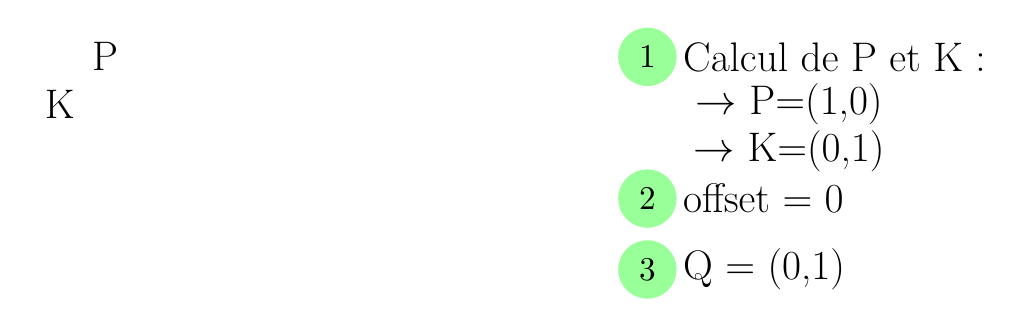
\begin{tikzpicture}[line cap=round,scale=0.6, every node/.style={transform shape}]
    \baseGraph
    \maze (-3,6) node {\BlueRoute}--(-3,5)node {\BlueRoute}; %ajouter ce qu'on a déjà fait 
    \draw (10,6) node[shape = circle,label=right:\Huge{Calcul de P et K :},fill=green!40,scale=2] {1}; \pause
    \draw (13,5) node {\Huge{$\rightarrow$ P=(1,0)}}; 
    \draw (-2,6) node[label=right:\Huge{P}] {\BlackCirc};\pause

    \draw (13,4) node {\Huge{$\rightarrow$ K=(0,1)}};
    \draw (-3,5) node[label=right:\Huge{K}] {\BlackCirc};\pause
    \draw (10,3) node[shape = circle,label=right:\Huge{offset = 0},fill=green!40,scale=2] {2};\pause
    \draw (10,1.5) node[shape = circle,label=right:\Huge{Q = (0,1)},fill=green!40,scale=2] {3}; 
    %\draw (-3,6) node {\BlueRoute}; \pause
\end{tikzpicture}
\end{frame}

\begin{frame}{Path merged : thread 1}
    \setbeamercovered{invisible}
\RaggedRight
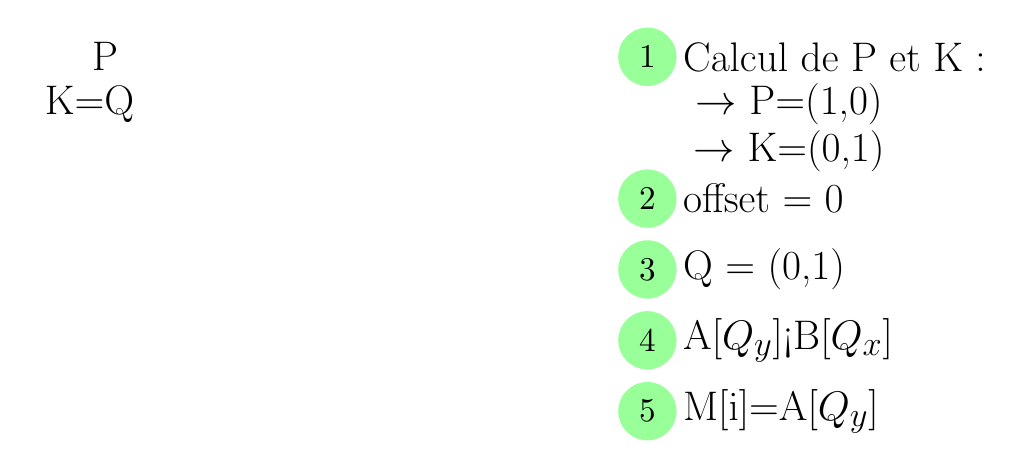
\begin{tikzpicture}[line cap=round,scale=0.6, every node/.style={transform shape}]
    \baseGraph
    \maze (-3,6) node {\BlueRoute}--(-3,5)node {\BlueRoute}; %ajouter ce qu'on a déjà fait 
    \draw (10,6) node[shape = circle,label=right:\Huge{Calcul de P et K :},fill=green!40,scale=2] {1}; 
    \draw (13,5) node {\Huge{$\rightarrow$ P=(1,0)}}; 
    \draw (-2,6) node[label=right:\Huge{P}] {\BlackCirc};

    \draw (13,4) node {\Huge{$\rightarrow$ K=(0,1)}};
    \draw (-3,5) node[label=right:\Huge{K=Q}] {\BlackCirc};
    \draw (10,3) node[shape = circle,label=right:\Huge{offset = 0},fill=green!40,scale=2] {2};
    \draw (10,1.5) node[shape = circle,label=right:\Huge{Q = (0,1)},fill=green!40,scale=2] {3};\pause
    \draw (10,0) node[shape = circle,label=right:\Huge{A[$Q_{y}$]<B[$Q_{x}$]},fill=green!40,scale=2] {4};\pause 
    \draw (10,-1.5) node[shape = circle,label=right:\Huge{M[i]=A[$Q_{y}$]},fill=green!40,scale=2] {5}; 
    %\draw (-3,6) node {\BlueRoute}; \pause
\end{tikzpicture}
\end{frame}


\begin{frame}{Path merged : thread 1, path}
    \setbeamercovered{invisible}
\RaggedRight
\begin{tikzpicture}[line cap=round,scale=0.6, every node/.style={transform shape}]
    \baseGraph
    \draw (-3,6) node {\BlueRoute}; 
    \maze (-3,6) node {\BlueRoute}--(-3,5)node {\BlueRoute};\pause
    \maze (-3,5) node {\BlueRoute}--(-3,4)node {\BlueRoute};
\end{tikzpicture}
\end{frame}